% Interposer Layer Stack Cross-Section (Slide 6)
\documentclass[border=3mm]{standalone}
\usepackage{tikz}
\usetikzlibrary{arrows.meta, positioning, calc, patterns}
\usepackage[T1]{fontenc}
\usepackage{lmodern}

\definecolor{IHPfg}{RGB}{0,80,139}
\definecolor{IHPaccent}{RGB}{109,112,114}
\definecolor{cM4}{RGB}{80,130,200}
\definecolor{cM5}{RGB}{50,160,200}
\definecolor{cTM1}{RGB}{60,170,100}
\definecolor{cTM2}{RGB}{200,60,60}
\definecolor{cVia}{RGB}{180,150,60}
\definecolor{cPass}{RGB}{160,160,165}
\definecolor{cSub}{RGB}{200,200,205}

\begin{document}
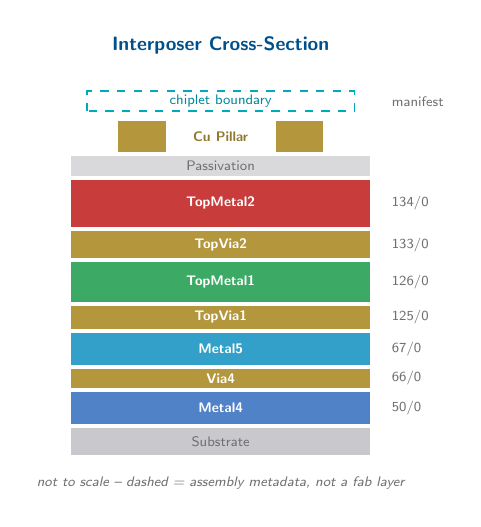
\begin{tikzpicture}[
    layer/.style={
        minimum width=38mm, minimum height=4mm,
        font=\sffamily\tiny\bfseries, text=white, align=center
    },
    via/.style={
        minimum width=38mm, minimum height=2.5mm,
        font=\sffamily\tiny, text=white, align=center,
        pattern=north east lines, pattern color=#1!60
    },
    lbl/.style={
        font=\sffamily\tiny, text=IHPaccent, anchor=west
    },
    brace/.style={
        decorate, decoration={brace, amplitude=3pt, mirror},
        line width=0.5pt, color=IHPaccent
    }
]

\def\W{3.8}  % layer width in cm
\def\y{0}    % running y position

% Substrate
\fill[cSub] (0, \y) rectangle (\W, \y+0.35);
\node[font=\sffamily\tiny, text=IHPaccent] at (\W/2, \y+0.175) {Substrate};
\pgfmathsetmacro{\y}{\y + 0.35 + 0.05}

% Metal4
\fill[cM4] (0, \y) rectangle (\W, \y+0.4);
\node[layer] at (\W/2, \y+0.2) {Metal4};
\node[lbl] at (\W+0.15, \y+0.2) {50/0};
\pgfmathsetmacro{\y}{\y + 0.4 + 0.05}

% Via4
\fill[cVia] (0, \y) rectangle (\W, \y+0.25);
\node[font=\sffamily\tiny\bfseries, text=white] at (\W/2, \y+0.125) {Via4};
\node[lbl] at (\W+0.15, \y+0.125) {66/0};
\pgfmathsetmacro{\y}{\y + 0.25 + 0.05}

% Metal5
\fill[cM5] (0, \y) rectangle (\W, \y+0.4);
\node[layer] at (\W/2, \y+0.2) {Metal5};
\node[lbl] at (\W+0.15, \y+0.2) {67/0};
\pgfmathsetmacro{\y}{\y + 0.4 + 0.05}

% TopVia1
\fill[cVia] (0, \y) rectangle (\W, \y+0.3);
\node[font=\sffamily\tiny\bfseries, text=white] at (\W/2, \y+0.15) {TopVia1};
\node[lbl] at (\W+0.15, \y+0.15) {125/0};
\pgfmathsetmacro{\y}{\y + 0.3 + 0.05}

% TopMetal1
\fill[cTM1] (0, \y) rectangle (\W, \y+0.5);
\node[layer] at (\W/2, \y+0.25) {TopMetal1};
\node[lbl] at (\W+0.15, \y+0.25) {126/0};
\pgfmathsetmacro{\y}{\y + 0.5 + 0.05}

% TopVia2
\fill[cVia] (0, \y) rectangle (\W, \y+0.35);
\node[font=\sffamily\tiny\bfseries, text=white] at (\W/2, \y+0.175) {TopVia2};
\node[lbl] at (\W+0.15, \y+0.175) {133/0};
\pgfmathsetmacro{\y}{\y + 0.35 + 0.05}

% TopMetal2
\fill[cTM2] (0, \y) rectangle (\W, \y+0.6);
\node[layer] at (\W/2, \y+0.3) {TopMetal2};
\node[lbl] at (\W+0.15, \y+0.3) {134/0};
\pgfmathsetmacro{\y}{\y + 0.6 + 0.05}

% Passivation
\fill[cPass!40] (0, \y) rectangle (\W, \y+0.25);
\node[font=\sffamily\tiny, text=IHPaccent] at (\W/2, \y+0.125) {Passivation};
\pgfmathsetmacro{\y}{\y + 0.25 + 0.05}

% Cu Pillar bumps (on top)
\fill[cVia] (0.6, \y) rectangle (1.2, \y+0.4);
\fill[cVia] (2.6, \y) rectangle (3.2, \y+0.4);
\node[font=\sffamily\tiny\bfseries, text=cVia!80!black] at (\W/2, \y+0.2) {Cu Pillar};
\pgfmathsetmacro{\y}{\y + 0.4 + 0.12}

% Chiplet boundary (assembly metadata, carried by the boundary manifest)
\definecolor{cExch}{RGB}{0,170,190}
\draw[cExch, dashed, line width=0.7pt]
    (0.2, \y) rectangle (\W-0.2, \y+0.25);
\node[font=\sffamily\tiny, text=cExch!80!black] at (\W/2, \y+0.125) {chiplet boundary};
\node[lbl] at (\W+0.15, \y+0.125) {manifest};
\pgfmathsetmacro{\y}{\y + 0.25}

% Title
\pgfmathsetmacro{\ytop}{\y + 0.15}
\node[font=\sffamily\scriptsize\bfseries, text=IHPfg, anchor=south]
    at (\W/2, \ytop+0.2) {Interposer Cross-Section};

% Scale note
\node[font=\sffamily\tiny\itshape, text=IHPaccent, anchor=north]
    at (\W/2, -0.15) {not to scale -- dashed = assembly metadata, not a fab layer};

\end{tikzpicture}
\end{document}
